% Options for packages loaded elsewhere
\PassOptionsToPackage{unicode}{hyperref}
\PassOptionsToPackage{hyphens}{url}
\PassOptionsToPackage{dvipsnames,svgnames,x11names}{xcolor}
%
\documentclass[
]{scrartcl}
\usepackage{amsmath,amssymb}
\usepackage{lmodern}
\usepackage{iftex}
\ifPDFTeX
  \usepackage[T1]{fontenc}
  \usepackage[utf8]{inputenc}
  \usepackage{textcomp} % provide euro and other symbols
\else % if luatex or xetex
  \usepackage{unicode-math}
  \defaultfontfeatures{Scale=MatchLowercase}
  \defaultfontfeatures[\rmfamily]{Ligatures=TeX,Scale=1}
\fi
% Use upquote if available, for straight quotes in verbatim environments
\IfFileExists{upquote.sty}{\usepackage{upquote}}{}
\IfFileExists{microtype.sty}{% use microtype if available
  \usepackage[]{microtype}
  \UseMicrotypeSet[protrusion]{basicmath} % disable protrusion for tt fonts
}{}
\makeatletter
\@ifundefined{KOMAClassName}{% if non-KOMA class
  \IfFileExists{parskip.sty}{%
    \usepackage{parskip}
  }{% else
    \setlength{\parindent}{0pt}
    \setlength{\parskip}{6pt plus 2pt minus 1pt}}
}{% if KOMA class
  \KOMAoptions{parskip=half}}
\makeatother
\usepackage{xcolor}
\IfFileExists{xurl.sty}{\usepackage{xurl}}{} % add URL line breaks if available
\IfFileExists{bookmark.sty}{\usepackage{bookmark}}{\usepackage{hyperref}}
\hypersetup{
  pdftitle={Übung: Pong},
  pdfauthor={Prof.~Dr.-Ing. Benedikt Dietrich; Prof.~Dr.~Martin Hobelsberger; Prof.~Dr.~Martin Orehek},
  pdflang={de},
  colorlinks=true,
  linkcolor={Maroon},
  filecolor={Maroon},
  citecolor={Blue},
  urlcolor={Blue},
  pdfcreator={LaTeX via pandoc}}
\urlstyle{same} % disable monospaced font for URLs
\usepackage{graphicx}
\makeatletter
\def\maxwidth{\ifdim\Gin@nat@width>\linewidth\linewidth\else\Gin@nat@width\fi}
\def\maxheight{\ifdim\Gin@nat@height>\textheight\textheight\else\Gin@nat@height\fi}
\makeatother
% Scale images if necessary, so that they will not overflow the page
% margins by default, and it is still possible to overwrite the defaults
% using explicit options in \includegraphics[width, height, ...]{}
\setkeys{Gin}{width=\maxwidth,height=\maxheight,keepaspectratio}
% Set default figure placement to htbp
\makeatletter
\def\fps@figure{htbp}
\makeatother
\setlength{\emergencystretch}{3em} % prevent overfull lines
\providecommand{\tightlist}{%
  \setlength{\itemsep}{0pt}\setlength{\parskip}{0pt}}
\setcounter{secnumdepth}{-\maxdimen} % remove section numbering
\ifLuaTeX
\usepackage[bidi=basic]{babel}
\else
\usepackage[bidi=default]{babel}
\fi
\babelprovide[main,import]{ngerman}
% get rid of language-specific shorthands (see #6817):
\let\LanguageShortHands\languageshorthands
\def\languageshorthands#1{}
\usepackage{fontawesome5}
\newcommand{\hint}{\faIcon{info}}
\newcommand{\warning}{\faIcon{exclamation-triangle}}
\newcommand{\task}{\faIcon{edit}}
\ifLuaTeX
  \usepackage{selnolig}  % disable illegal ligatures
\fi

\title{\includegraphics[height=2cm]{HM_Schriftzug_Logo_rot_RGB} \\[\bigskipamount]Übung:
Pong}
\usepackage{etoolbox}
\makeatletter
\providecommand{\subtitle}[1]{% add subtitle to \maketitle
  \apptocmd{\@title}{\par {\large #1 \par}}{}{}
}
\makeatother
\subtitle{Computational Thinking}
\author{Prof.~Dr.-Ing. Benedikt Dietrich \and Prof.~Dr.~Martin
Hobelsberger \and Prof.~Dr.~Martin Orehek}
\date{}

\usepackage[outputdir=temp]{minted}

\begin{document}
\maketitle

\hypertarget{disclaimer}{%
\section{Disclaimer}\label{disclaimer}}

In diesem Übungsblatt werden folgende Symbole verwendet:

\begin{itemize}
\tightlist
\item
  \faIcon{info} FYI - Hier erhalten sie weiterführende, informative
  Hinweise.
\item
  \faIcon{exclamation-triangle} Wichtige Inhalte - hier ist aufmerksames
  Lesen geboten.
\item
  \faIcon{edit} Hier müssen Sie aktiv werden - Es folgen Aufgaben, die
  Sie bearbeiten sollen.
\end{itemize}

\hypertarget{pygame}{%
\section{Pygame}\label{pygame}}

Im Rahmen dieser Übung verwenden wir die Spiele-Bibliothek
\texttt{pygame}. Diese ist im Vergleich zu modernen
Spieleentwicklungsplattformen wie Unity eher rudimentär ausgestattet.
Dafür ist \texttt{pygame} auf Grund der Einfachheit gut geeignet die
grundlegenden Konzepte von Computerspielen zu verstehen.

\hypertarget{pong}{%
\section{Pong}\label{pong}}

In dieser Übung soll das Spiel Pong entwickelt werden. Bei diesem
Klassiker fliegt ein Ball durch das Spielfeld. Jeder Spieler hat ein
Paddel, das er mit Hilfe der Tastatur nach oben, oder unten bewegen
kann. Ziel ist es den Ball 10 Mal hinter das gegnerische Paddel zu
bringen. Folgender Screenshot zeigt das Endergebnis der Entwicklung:

\begin{figure}
\centering
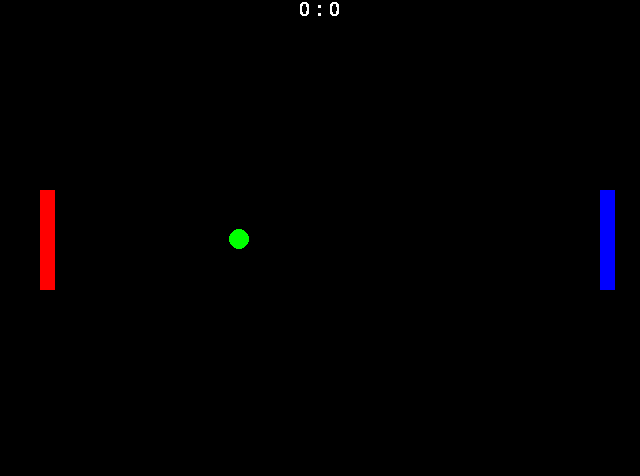
\includegraphics[width=0.6\textwidth,height=\textheight]{/tmp/tex2pdf.-d16cf184ed2bc795/images/screenshot.png}
\caption{So sollte Ihr Spiel am Ende aussehen}
\end{figure}

\hypertarget{divide-and-conquer}{%
\subsection{Divide and Conquer}\label{divide-and-conquer}}

Diese Aufgabe ist durchaus komplex, kann aber durch die Aufteilung des
Problems in Einzelschritte von Ihnen gelöst werden.

Die Einzelschritte sind gegeben durch:

\begin{enumerate}
\def\labelenumi{\arabic{enumi}.}
\tightlist
\item
  Diagonale Bewegung des Balls
\item
  Geschwindigkeit des Balls
\item
  Abprallen des Balls an der Wand
\item
  Aktualisierung der Ball-Position auf Basis der vergangenen Zeit
\item
  Erstellen eines \texttt{ball} Dictionaries
\item
  Refaktorisieren in Funktionen
\item
  Zeichnen eines Paddels an eine feste Position
\item
  Bewegung eines Paddels mittels Tastatur
\item
  Kollisionsprüfung mit Paddel
\item
  Erweiterung um das zweite Paddel
\item
  Ermitteln und Anzeigen der Score
\end{enumerate}

\hypertarget{diagonale-bewegung-des-balls}{%
\subsection{Diagonale Bewegung des
Balls}\label{diagonale-bewegung-des-balls}}

Gegeben ist ein Programm, welches aktuell

\begin{itemize}
\tightlist
\item
  \texttt{pygame} initialisiert,
\item
  ein Fenster einer definierten Größe erstellt,
\item
  bestimmte Events behandelt und
\item
  einen Kreis an eine feste Position zeichnet.
\end{itemize}

\faIcon{edit} Lesen Sie zunächst den gegebenen Source Code und verstehen
Sie die einzelnen Teile. Bemühen Sie hierzu auch die Vorlesungsfolien.

\faIcon{edit} Führen Sie zwei Variablen \texttt{ball\_position\_x} und
\texttt{ball\_position\_y} ein, welche die x- und die y-Koordinaten des
Ballmittelpunkts speichern. Verwenden Sie die neuen Variablen beim
Zeichnen des Kreises. Erweitern Sie das Programm nun so, dass sich der
Ball bei jedem Schleifendurchlauf (d.h. pro Frame) um zehn Pixel nach
rechts und zehn Pixel nach unten bewegt.

Der Ball sollte nun diagonal nach rechts unten fliegen. Der Ball
verlässt aktuell noch den Bildausschnitt.

\hypertarget{eine-geschwindigkeit-fuxfcr-den-ball}{%
\subsection{Eine Geschwindigkeit für den
Ball}\label{eine-geschwindigkeit-fuxfcr-den-ball}}

\faIcon{edit} Definieren Sie nun zwei Variablen \texttt{ball\_speed\_x}
und \texttt{ball\_speed\_y}, welche die Geschwindigkeit in x- und
y-Richtung speichern. Beide Variablen sollen zu Beginn den Wert
\texttt{10} haben (die Einheit ist noch Pixel pro Frame). Verwenden Sie
die Variablen an den Stellen, an denen Sie die neue Position des Balls
berechnen.

\hypertarget{abprallen-des-balls}{%
\subsection{Abprallen des Balls}\label{abprallen-des-balls}}

In dieser Teilaufgabe soll nun verhindert werden, dass der Ball aus dem
Bildbereich fliegt.

\faIcon{edit} Kehren Sie die x-Geschwindigkeit des Balls um (Änderung
des Vorzeichens), wenn die x-Position des Balls größer ist, als das
Fenster breit ist, bzw. die x-Position des Balls kleiner als null ist.
Die Breite des Fensters ist gegeben mit \texttt{WINDOW\_WIDTH}.

\faIcon{edit} Führen Sie die gleichen Überprüfungen für die y-Koordinate
ein. Die Höhe des Fensters ist gegeben mit \texttt{WINDOW\_HEIGHT}.

Nun sollte der Ball durch das Fenster fliegen und an den Rändern
abprallen. Ein Problem ist aber vermutlich noch, dass der Ball immer
noch kurz teilweise am Bildschirmrand eintaucht. Das liegt daran, dass
\texttt{ball\_position\_x} und \texttt{ball\_position\_y} den
Mittelpunkt des Kreises beschreiben. Die Abbildung \ref{fig:collision}
zeigt den Zeitpunkt, zu dem der Ball den rechten Rand berührt und auch
abprallen sollte.

\begin{figure}
\centering
\includegraphics{/tmp/tex2pdf.-d16cf184ed2bc795/41e38e8df70b614a1424792784158cb3f43af076.pdf}
\caption{\label{fig:collision}Ball berührt die Wand}
\end{figure}

\faIcon{edit} Überlegen Sie sich (z.B. auf auf einem Blatt Papier), wie
Sie Ihre Überprüfung der Position erweitern müssen, sodass der Radius
des Balls berücksichtigt wird. Erweitern Sie das Programm entsprechend,
sodass der Ball auf keiner Seite mehr eintaucht.

\hypertarget{beruxfccksichtigung-der-vergangenen-zeit}{%
\subsection{Berücksichtigung der vergangenen
Zeit}\label{beruxfccksichtigung-der-vergangenen-zeit}}

Wie in der Vorlesung besprochen kann der aktuelle Code dazu führen, dass
der Ball sich ungleichmäßig bewegt und die Bewegung je nach PC
unterschiedlich schnell abläuft.

Die Funktion \texttt{clock.tick(60)} liefert die vergangene Zeit seit
dem letzten Aufruf der Funktion zurück. Die Einheit von
\texttt{delta\_t} ist Millisekunden.

\faIcon{edit} Ändern Sie die zwei Variablen \texttt{ball\_speed\_x} und
\texttt{ball\_speed\_y} ab und weisen ihnen jeweils den Wert
\texttt{150} zu.

\faIcon{edit} Berechnen Sie die aktuelle Position des Balls auf Basis
der aktuellen Geschwindigkeit (\texttt{ball\_speed\_x} und
\texttt{ball\_speed\_y}), der vergangenen Zeit \texttt{delta\_t} und der
aktuellen Position (\texttt{ball\_position\_x} und
\texttt{ball\_position\_y}). Sie finden hierzu einige Informationen in
den Vorlesungsfolien.

\faIcon{exclamation-triangle} Die Einheit von \texttt{ball\_position\_x}
und \texttt{ball\_position\_y} ist Pixel pro Sekunde. Die Einheit von
\texttt{delta\_t} ist Millisekunden. Die Einheit von
\texttt{ball\_position\_x} und \texttt{ball\_position\_y} ist Pixel.

Der Ball sollte sich nun nach wie vor im Fenster bewegen und an den
Fensterrändern abprallen. Der Unterschied ist, dass die Geschwindigkeit
in der Einheit Pixel pro Sekunde angegeben wird und nicht mehr in Pixel
pro Frame. Somit sollte die Animation auf jedem PC gleich schnell
ablaufen.

\newpage

\hypertarget{sammeln-der-eigenschaften-in-einem-dictionary}{%
\subsection{Sammeln der Eigenschaften in einem
Dictionary}\label{sammeln-der-eigenschaften-in-einem-dictionary}}

Wenn wir so weiterprogrammieren wie bisher, haben wir in unserem
Programm bald sehr schnell sehr viele einzelne Variablen. Viele dieser
Variablen gehören thematisch zusammen.

Der Ball wird im Spiel folgende Eigenschaften haben:

\begin{itemize}
\tightlist
\item
  \emph{position}: Position des Balls als Liste, wobei der erste Eintrag
  der x-Koordinate des Balls entspricht und der zweite Eintrag der
  y-Koordinate.
\item
  \emph{speed}: Geschwindigkeit des Balls (und damit auch Richtung) als
  Liste. Der erste Eintrag entspricht der Geschwindigkeit in x-Richtung,
  der zweite Wert der Geschwindigkeit in y-Richtung.
\item
  \emph{radius}: Der Radius des Balls, z.B. \texttt{10}.
\item
  \emph{color}: Die Farbe des Balls als RGB-Tupel.
  \texttt{(0,\ 255,\ 0)} entspricht z.B. der Farbe Grün.
\end{itemize}

Wir wollen alle diese Eigenschaften in einem Dictionary (Wörterbuch)
namens \texttt{ball} bündeln. Folgender Code zeigt anhand der
Eigenschaft \texttt{position}, wie das gemeint ist:

\begin{minted}{python}
ball = {
    "position": [50.0, 50.0] # center
}
\end{minted}

\faIcon{edit} Erweitern Sie den Code um die geforderten restlichen
Eigenschaften. Verwenden Sie die neue Datenstruktur in Ihrem Programm
und ersetzen Sie \texttt{ball\_position\_x}, \texttt{ball\_position\_y},
\texttt{ball\_speed\_x} und \texttt{ball\_speed\_y} in Ihrem Programm
mit der neuen Datenstruktur.

\textbf{Achtung Spoiler:}

\texttt{ball\_position\_x} muss dann z.B. durch
\texttt{ball{[}"position"{]}{[}0{]}} ersetzt werden.

\hypertarget{auslagern-in-funktionen}{%
\subsection{Auslagern in Funktionen}\label{auslagern-in-funktionen}}

Ihre \texttt{main}-Funktion ist mittlerweile schon deutlich zu lang
geworden. Es sollen nun Teile in Funktionen ausgelagert werden, um so
den Code wieder übersichtlicher zu machen und Details zu abstrahieren.

\faIcon{info} Erstellen Sie vor der Umstrukturierung eine
Sicherheitskopie von Ihrem Code. So können Sie jederzeit zum
ursprünglichen Code zurückkehren.

\faIcon{edit} Definieren Sie zwei Funktionen und lagern Sie den
entsprechenden Code aus der \texttt{main} in die Funktionen aus:

\begin{itemize}
\tightlist
\item
  \texttt{update\_ball}: Bekommt \texttt{delta\_t} und \texttt{ball}
  übergeben und aktualisiert in \texttt{ball} die Position. In der
  Funktion wird auch die Kollision mit den Wänden geprüft.
\item
  \texttt{draw\_ball}: Bekommt \texttt{screen} und \texttt{ball}
  übergeben und zeichnet den Ball anhand der Eigenschaften von
  \texttt{ball}.
\end{itemize}

Jetzt sollte Ihre Hauptschleife wieder deutlich übersichtlicher sein.
Das Verhalten sollte sich natürlich durch die Umstrukturierung nicht
geändert haben.

\hypertarget{das-erste-paddel}{%
\subsection{Das erste Paddel}\label{das-erste-paddel}}

Analog zu \texttt{ball} hat ein Paddel folgende Eigenschaften:

\begin{itemize}
\tightlist
\item
  \emph{position}: Position des Paddels als Liste, wobei der erste
  Eintrag der x-Koordinate der linken, oberen Ecke des Paddels
  entspricht und der zweite Eintrag der y-Koordinate der linken, oberen
  Ecke des Paddels.
\item
  \emph{speed}: Geschwindigkeit des Paddels (und damit auch Richtung)
  als Liste. Der erste Eintrag entspricht der Geschwindigkeit in
  x-Richtung, der zweite Wert der Geschwindigkeit in y-Richtung. Das
  Paddel soll sich aber nur in y-Richtung bewegen können, d.h. die
  x-Koordinate wird immer \texttt{0} sein.
\item
  \emph{width}: Breite des Paddels, z.B. \texttt{15}.
\item
  \emph{height}: Höhe des Paddels, z.B. \texttt{100}.
\item
  \emph{color}: Die Farbe des Balls als RGB-Tupel.
  \texttt{(255,\ 0,\ 0)} entspricht z.B. der Farbe Rot.
\end{itemize}

Folgende Grafik zeigt wie die Koordinaten zu verstehen sind:

\begin{figure}
\centering
\includegraphics[width=0.3\textwidth,height=\textheight]{/tmp/tex2pdf.-d16cf184ed2bc795/e22d108891c539e2d0b4fbed9648e90b973c533a.pdf}
\caption{Koordinaten des Paddels}
\end{figure}

\faIcon{edit} Erstellen Sie analog zu \texttt{ball} das Dictionary
\texttt{paddle1} für das linke Paddel. Das Paddel soll zu Beginn
vertikal zentriert sein. Der Abstand vom linken Fensterrand soll 40
Pixel groß sein.

\faIcon{edit} Schreiben Sie eine Funktion \texttt{draw\_paddel}, welcher
\texttt{screen} und das Dictionary \texttt{paddle} übergeben wird. Die
Funktion soll das Rechteck basierend auf den im Dictionary enthaltenen
Daten in das Fenster zeichnen.

\hypertarget{move-it}{%
\subsection{Move it!}\label{move-it}}

Im nächsten Schritt wollen wir Spieler 1 ermöglichen, das Paddel zu
bewegen.

\faIcon{edit} Erweitern Sie die Funktion \texttt{handle\_keys} um den
Übergabeparameter \texttt{paddle1}. Reagieren Sie in der Funktion auf
Tastendrücke wie folgt:

\begin{itemize}
\tightlist
\item
  wird \texttt{pygame.K\_UP} gedrückt, soll die Geschwindigkeit von
  \texttt{paddle1} auf \texttt{-200} gesetzt werden. Wird die Taste
  wieder losgelassen soll die Geschwindigkeit auf \texttt{0} gesetzt
  werden.
\item
  wird \texttt{pygame.K\_DOWN} gedrückt, soll die Geschwindigkeit von
  \texttt{paddle1} auf \texttt{200} gesetzt werden. Wird die Taste
  wieder losgelassen soll die Geschwindigkeit auf \texttt{0} gesetzt
  werden.
\end{itemize}

Nun sollte durch das Drücken der Tasten die Geschwindigkeit des Paddels
beeinflusst werden können. Damit sich das Paddel auch bewegt müssen wir
die Position des Paddels noch aktualisieren.

\faIcon{edit} Schreiben Sie eine Funktion \texttt{update\_paddle},
welcher \texttt{delta\_t} und \texttt{paddle} übergeben werden. In der
Funktion soll die Position des Paddels auf Basis der vergangenen Zeit
und der Geschwindigkeit des übergebenen Paddels aktualisiert werden.
Überlegen Sie sich außerdem, wie sie verhindern können, dass das Paddel
aus dem Fenster herausbewegt werden kann. Implementieren Sie Ihre Idee.

\hypertarget{kollision-mit-dem-paddel}{%
\subsection{Kollision mit dem Paddel}\label{kollision-mit-dem-paddel}}

Aktuell fliegt der Ball einfach durch das Paddel hindurch. Das wollen
wir in dieser Aufgabe ändern.

Im Modul \texttt{collision.py} existiert hierfür bereits eine Funktion
\texttt{get\_collision\_side}. Mit Hilfe dieser Funktion können Sie
bestimmen, auf welcher Seite der Ball mit dem Paddel kollidiert. Die
Funktion liefert entweder \texttt{"left"}, \texttt{"right"},
\texttt{"top"}, \texttt{"bottom"} oder, falls Ball und Paddel sich nicht
berühren, \texttt{"none"} zurück.

\faIcon{edit} Erweitern Sie die Funktion \texttt{update\_ball} um den
Übergabeparameter \texttt{paddle1}. Bestimmen Sie die Seite der
Kollision und reagieren Sie wie folgt:

\begin{itemize}
\tightlist
\item
  Kehren Sie die Geschwindigkeit des Balls im Falle einer Kollision um
  (x- oder y-Richtung, je nach Kollisionsseite).
\item
  Setzen Sie die Position des Balls auf die Kollisionsseite des Paddels,
  aber außerhalb mit kleinem Sicherheitsabstand (z.B. \texttt{5} Pixel).
  Damit vermeiden Sie, dass der Ball in das Paddel eintaucht und dann am
  Paddel kleben bleibt.
\item
  Nur wenn keine Kollision vorliegt, soll die Position des Balls um die
  auf Basis von \texttt{ball{[}"speed"{]}} und \texttt{delta\_t}
  berechnete Strecke verändert werden.
\end{itemize}

Eventuell bedarf der implementierte Algorithmus etwas Fine-Tuning.
Testen Sie ausgiebig.

\hypertarget{ein-paddel-kommt-selten-allein}{%
\subsection{Ein Paddel kommt selten
allein}\label{ein-paddel-kommt-selten-allein}}

\faIcon{edit} Erweitern Sie nun den Code um das zweites Paddel
\texttt{paddle2}. Beachten Sie, dass nur die Funktionen
\texttt{handle\_keys} und \texttt{update\_ball} jeweils \texttt{paddle2}
als zusätzlichen Übergabeparameter brauchen. Die anderen Funktionen
sollten einfach zweimal aufgerufen werden können: einmal mit
\texttt{paddle1} und einmal mit \texttt{paddle2}.

\faIcon{info} Verwenden Sie z.B. die Tasten \texttt{pygame.K\_w} und
\texttt{pygame.K\_s} für das zweite Paddel.

\hypertarget{score-anzeigen}{%
\subsection{Score anzeigen}\label{score-anzeigen}}

Um in Pygame Text auszugeben, muss man zunächst eine Schrift laden. Das
macht man einmal, d.h. oberhalb der Hauptschleife:

\begin{minted}{python}
my_font = pygame.font.SysFont('Comic Sans MS', 30)
\end{minted}

Nun kann man bei jedem Schleifendurchlauf einen Schriftzug in einen
separaten Grafikspeicher zeichnen und diesen dann an die gewünschte
Stelle im Fenster kopieren (auch blitting genannt):

\begin{minted}{python}
text_surface = my_font.render("0 : 0", False, (255, 255, 255))
screen.blit(text_surface, (0,0))
\end{minted}

\faIcon{edit} Erweitern Sie das Spiel um die Anzeige der Score. Die
Anzeige soll horizontal zentriert im oberen Bereich erscheinen und den
Spielstand (z.B. \texttt{4\ :\ 3}) anzeigen.

\faIcon{info} Sie können die Breite des gerenderten Textes mittels
\texttt{text\_surface.get\_width()} herausfinden.

\faIcon{edit} Prüfen Sie die Position des Balls: ist der Ball hinter dem
linken oder rechten Paddel soll die Score des jeweiligen Spielers erhöht
werden. Der Ball soll in die Mitte des Fensters zurückgesetzt werden.
Das Spiel soll direkt weitergehen.

\hypertarget{lets-play}{%
\subsection{Let’s Play}\label{lets-play}}

Glückwunsch! Sie sollten nun Ihr erstes grafisches Computerspiel
programmiert haben.

\end{document}
